%
% File hicss51.tex
%
% Contact: Holm Smidt, hsmidt@hawaii.edu
%%
%%
%% Based on the style files for ACL 2015 by 
%% car@ir.hit.edu.cn, gdzhou@suda.edu.cn


\documentclass[10pt]{article}
\usepackage[letterpaper]{geometry}
\usepackage{hicss51}
\usepackage{times}
\usepackage[none]{hyphenat}
\usepackage{url}
\usepackage{latexsym}
\usepackage{minted}
\usepackage{indentfirst}
\usepackage{graphicx}
\usepackage{datetime}
\usepackage{cite}
\usepackage[hyphens]{url}
\usepackage[hidelinks]{hyperref}
\usepackage{csquotes}
\usepackage{array}
\usepackage{multirow}
\usepackage{multicol}
\usepackage{pdflscape}
\usepackage{amsmath}
\usepackage{float}
\usepackage{afterpage}
\hypersetup{breaklinks=true}
\newcommand{\subparagraph}{}
\usepackage{titlesec}
\setcounter{secnumdepth}{4}
\graphicspath{{images/}}

\newcommand{\sansserifformat}[1]{\fontfamily{cmss}{ #1}}%

%\setlength\titlebox{5cm}

% You can expand the titlebox if you need extra space
% to show all the authors. Please do not make the titlebox
% smaller than 5cm (the original size).


\title{Please Read Carefully Detailed Formatting Guidelines for Preparing Your HICSS Final Paper with Author Names}

\author{First Author \\
  Affiliation \\
  {\underline{ email@domain}} \\\And
  Second Author \\
  Affiliation \\
  {\underline{ email@domain} }\\\And 
  Third Author \\
  Affiliation \\
  {\underline{email@domain}} \\}

\date{}

\begin{document}
\maketitle
\begin{abstract}


\end{abstract}

\section{Introduction}
With the pervasiveness of technology users today disclose a huge amount of personal information, such as their address, credit card and banking details and even their health conditions, into software systems on a daily basis. For example, every time you shop and tap your credit card into the payment system, you disclose what you bought, and what you paid into the system. The system can very easily do some processing with this data and let the shop know your preferred brands, your weekly expenditure on groceries and predict how to target you with advertising. Therefore, when users disclose more data into software applications, the ways through which user privacy could be compromised through these software systems increase. 

Disclosure of personal details always comes with an associated privacy risk that concerns users. Users are known to be reluctant to disclose data when the associated privacy risk is high \cite {kobsa2007privacy}, because using data for reasons unforeseen by users and sharing data with third parties unknown to the user could result in privacy vulnerabilities \cite {malhotra2004internet}. Furthermore, the uncertainty of the consequences of the decision also adds to the complexity of making the disclosure decision due to increased privacy risk \cite {knijnenburg2013helping}. Disclosure decisions of users are closely related to privacy as users disclose data when their perceived privacy risk is low. For example, higher discomfort in disclosing data implies a higher privacy risk. Therefore, understanding data disclosure decisions made by users could help understanding perceived privacy risk by users.


Privacy conscious users face many problems when they make decisions to disclose their information into software systems \cite {li2010understanding}. Current approaches to observe user data disclosure decisions focus either on the properties of the application that request data \cite {li2010understanding, wang2016context, malheiros2013fairly} or the personality aspects of the user who disclose data \cite {nissenbaum2009privacy}. The effect of the properties of data itself such as : How sensitive is this data? Who can view this data in this application? How relevant is this data to the application? also have an effect on the disclosure decisions of users. However, the apparent effect these concerns have on the disclosure decisions of the user is not directly observable. Lack of understanding about the aspects of data that concern users when they disclose data makes it difficult for privacy researchers and software developers to implement user privacy preferences when they design software systems. 

Knowledge of the effect of the properties of data being collected on the data disclosure decisions of users could help building up a metric for privacy risk of data items. In order to ensure user privacy preferences are met, developers need to be able to measure and quantify the privacy risk of certain data items are for users. When a developer can measure and quantify privacy of the data they utilize in a system, they can decide which data to collect, which data to store and how to store and process user data in the system. Similarly, with a privacy measurement researchers and law makers can make better regulations and privacy practices that would enable developers to understand data from a user perspective to design privacy preserving software systems. However, in order to make a privacy risk measurement for data, first one needs to identify the factors that affect privacy of data items for a user and the relationship among these factors. For example, would users be more comfortable sharing their credit card number with their banking application than their social networking account? Would users be equally comfortable sharing their blood group with their banking application? Would users be more comfortable sharing their age than their birthday with their social networking account? 

In this research we attempt to extract how users perceive different aspects of data that leads to their decisions in disclosing their data into software systems. Our goal is to identify the relationship among these parameters in order to obtain a privacy risk metric for different data items in different application settings. Using a survey with 151 respondents we observe how users perceive the sensitivity of the data items to the user, relatedness of the data items to the purpose of an application and the visibility a particular data item gets in an application when they decide to disclose their data into software systems. With this knowledge we attempt to build a relationship relating how sensitivity, visibility and relatedness of data items relate to user privacy risk. We measure perceived privacy risk when users disclose their data items in different settings. Furthermore, through a qualitative analysis we attempt to identify other factors, if any, that could affect users data disclosure decisions.

This paper has two contributions.

\begin{itemize}
\item  First, measure privacy of data disclosure decisions. A metric to measure privacy that takes into account the context in which it is disclosed (by considering the relatedness of the data item to the application context) would help software developers to make decisions about collecting, storing and using different data items in software systems. 
\item Second, understanding factors that affect users' data disclosure decisions. Understanding factors that affect users' decisions to disclose their data into software systems would help organizations to build positive relationships with users when they collect user data for different services and business purposes. 
\end{itemize}

The paper is structured as follows. We first discuss previous work that has identified the parameters (sensitivity, visibility and relatedness) in measuring privacy in the background section. Then we describe our user study followed by the results. Next, we discuss the implicatins of our findings followed by the conclusion and future work.

\section {Related work}

Most research that focus on user disclosure decisions have the motivation to increase user data disclosure. These research focus on what makes users disclose more data rather than understanding how users disclose data. For example, Besmer et al. said that users are more likely to decide to disclose data when they are shown the decisions made by other users \cite {besmer2010impact} Similarly, Dennett has said that users feel comfortable sharing their data when they are shown the decisions made by their friends. \cite {dennett2000little}. Furthermore, Acquisti et al. found that changing the order of intrusiveness of the data being requested also makes users disclose more data when interacting with software systems \cite {acquisti2012impact}. Similarly, testing the effect of the justification provided by the system when requesting data Knijnenburg and Kobsa \cite {knijnenburg2013helping} revealed that when users are told \textit{this data is useful for you} users are more likely to disclose data with the application. Interestingly, all these research focus on system behaviors (way of requesting data, justification for data collection) and user's personal preferences ( users' experience with a system, users' expectation from a system) and their effects on user data disclosure decisions.

Particularly focusing on the intrinsic properties of the data being shared, Bansal et al. have shown that users' intention to disclose health information is affected by the sensitivity of the data\cite {bansal2010impact}. Previous work has shown that consumer willingness to share personal data is affected by the sensitivity of the data \cite {malhotra2004internet}. Malheiros et al. \cite {malheiros2013fairly} have shown that sensitivity of data items such as date of birth and occupation had a significant affect on disclosure. 

Particularly focusing on privacy risk, Maximilien et al. \cite {maximilien2009privacy} have shown that a metric for privacy in a given context can be obtained by multiplying the measurement for sensitivity of a data item with the measurement for visibility the data item gets in an application. They define their metric for privacy as \enquote{a measurement that determines their [the user's ]willingness to disclose information associated with this item} \cite {maximilien2009privacy}. Using the same metric, Minkus and Memon \cite{minkus2014scale} have attempted to measure user privacy from their Facebook privacy settings. They have shown that the metric could be used to measure the privateness of a user from the choices s/he makes when setting up the privacy settings in Facebook. However, this is a contextual measurements. The context in which data is being disclosed \cite {nissenbaum2009privacy, john2010strangers} is also known to have an effect on user disclosure decisions \cite {knijnenburg2013making}. For example, it is said that users have an undermining effect on rewards for data disclosure when the requested data appears irrelevant for a system \cite {li2010understanding}, whereas they accepted the rewards if the data is relevant for the system. Therefore, a holistic measurement for privacy needs to consider all these factors when measuring user privacy from the data disclosure decisions. 

We focus on investigating the effect of sensitivity, the relevance of the data for an application and the visibility the data gets in the application to user disclosure decisions. With this we focus on obtaining a privacy risk metric in order to communicate the effect of data sensitivity, visibility and the relatedness of data for a particular application on user disclosure decisions to software developers and privacy researchers. This metric would help software developers to understand and incorporate user disclosure decisions into the software system designs and assist the development of privacy preserving software systems


\section {Research Methodology}

Our goal in this research is to understand how sensitivity, visibility and relatedness affect associated privacy risk of a data item. Going along with Maximilien et al. we define privacy risk to be \enquote{a measurement that determines the user's comfortability in disclosing information associated with this item} \cite {maximilien2009privacy}. We conduct a user survey to understand user decision making when they disclose their personal data into software systems. For this, we conducted an online survey with 151 users. We designed the survey with 4 simple questions with Likert scales. We used a list of 10 data items and four different mobile application contexts in the questionnaire. The application context we defined were,

\begin{itemize}
\item Undefined application
\item Health Care application
\item Social Networking application - with no control over data visibility (Cannot control who can view the data once disclosed)
\item Banking application
\end{itemize}

We defined the data items including demographic data and sensitive data following the Data Protection Regulations. The data items we provided are name, age, address, mobile number, email address, occupation, blood type, credit card number, medicine taken, and birthday. We asked the participants how they would feel if they are to disclose the 10 data items in the four application contexts. We define this feeling as the \textit{feeling of disclosure} $F_d$. We used a five point Likert scale with values, very uncomfortable, somewhat uncomfortable, neutral, somewhat comfortable and very comfortable for users to express their feelings. We consider $F_d$ to be a function of sensitivity ($D_s$) and visibility ($D_v$) of the data item and the relatedness of the data item to the context of the software system ($D_r$). Our goal is to determine how $D_s$, $D_v$ and $D_r$ affect $F_d$.

Following these four questions we also included an open ended question in the questionnaire to identify any factors other than what we explicitly investigated in the survey, that could affect users data disclosure decisions when they interact with software systems. 

At the end of the survey, we included questions to extract the demographics of the participants. However, we included an option \textit{prefer not to say} in all these questions, so that users could avoid disclosing their age, gender and educational background.

Following is the basic profile of the participants;

\begin{center}
\begin{table}[htbp]
\caption{Participant Gender Distribution}
\begin{center}
\begin{tabular}{|l|l|} 
\hline
Gender & No. of Participants \\
\hline
Male & 87 \\
\hline
Female & 64 \\
\hline
\end{tabular}
\end{center}
\end{table}
\end{center} 

\begin{center}
\begin{table}[htbp]
\caption{Participant Education Distribution}
\begin{center}

\begin{tabular}{|l|l|} 
\hline
Education & No. of Participants \\
\hline
Completed School Education & 5 \\
\hline
Professional Diploma & 9 \\
\hline
Bachelor's Degree & 87 \\
\hline
Masters/PhD & 50 \\
\hline
\end{tabular}
\end{center}
\end{table}
\end{center} 

\begin{center}
\begin{table}[htbp]
\caption{Participant Age Distribution}
\begin{center}
\begin{tabular}{|l|l|} 
\hline
Age & No. of Participants \\
\hline
18-24  & 31 \\
\hline
25-32 & 101 \\
\hline
33-40& 13 \\
\hline
41 or above & 6\\
\hline
\end{tabular}
\end{center}
\end{table}
\end{center} 

The survey design was evaluated with two participants (graduate students in the university not connected to the research). We fine tuned the wording of the questionnaire with the feedback of these two participants. Then the survey was distributed using social media platforms (Facebook, LinkedIn and Twitter) and personal connections of the authors. Before proceeding to the survey, participants were given a brief introduction about the survey and the duration of the survey (under 10 minutes, calculated using the participants who evaluated the questionnaire). We also provided the participants with the contact details of the researchers. The research methodology (survey design, participant recruitment and results collection) was approved by the university ethic committee responsible for ethical conduction of studies that involve human subjects.

We measured the participant adequacy while collecting data and stopped data collection once we reached sample adequacy at KMO = 0.8. We then analyzed the data to obtain results.

\subsection {Data Analysis}

We assigned values from 1 to 5 for the answers we received on the Likert scale as follows.

\begin{center}
\begin{table}[htbp]
\caption{Assigning values to Likert Scale preferences}
\begin{center}
\begin{tabular}{|l|l|} 
\hline
Likert Scale Preference & Value Assigned \\
\hline
Very Comfortable & 1\\
\hline
Somewhat Comfortable& 2 \\
\hline
Neutral & 3  \\
\hline
Somewhat Uncomfortable & 4 \\
\hline
Very Uncomfortable & 5 \\
\hline
\end{tabular}
\end{center}
\end{table}
\end{center}

The goal of our research was to calculate the relationship between sensitivity, relatedness and visibility of data when users make their disclosure decisions. The data we collected in the study was the feeling of disclosure of data by participants in different scenarios. From this we first calculate the
\begin{itemize}
\item Effect of data sensitivity to the feeling of disclosure -  $F_d,D_s$, 
\item Effect of data visibility to the feeling of disclosure -  $F_d,D_v$, 
\item Effect of data relatedness to the feeling of disclosure -  $F_d,D_r$, 
\end{itemize}

for each participant when they disclose data into software applications. This calculation was done as follows.

\[ \begin{aligned} \text{Effect of } \\ \text{Sensitivity}(F_{d}, D_{s}) \end{aligned} =
\frac{\begin{aligned}
      \text{Sharing a sensitive data item } \\ \text{ in an application}
      \end{aligned}}%
 {\begin{aligned}
      \text{Sharing a not so sensitive data item }\\ \text{ in the same application}
      \end{aligned}}
\]

We defined sensitive elements following the European Data Protection Regulation's definition for the data analysis. According to their definition we identified, user's credit card details, user's health information (subscribed medicine, blood type) as sensitive data and user's name as a not so sensitive data item. 

Similarly, we calculated $F_d,D_v$ and $F_d,D_r$,

\[ \begin{aligned} \text{Effect of } \\ \text{Visibility}\\ (F_{d},D_{v}) \end{aligned} =
\frac{\begin{aligned}
      \text{Sharing a data item in an application where } \\ \text{ the user cannot control the visibility} \\ \text{of the data item}
      \end{aligned}}%
 {\begin{aligned}
       \text{Sharing a data item in an application where } \\ \text{ the user can control the visibility} \\ \text{of the data item}
      \end{aligned}}
\]



\[ \begin{aligned} \text{Effect of } \\ \text{Relatedness}(F_{d},D_{r})\end{aligned} =
\frac{\begin{aligned}
      \text{Sharing a related data item} \\ \text{  with an application}
      \end{aligned}}%
 {\begin{aligned}
      \text{Sharing an unrelated data item }\\ \text{with the same application}
      \end{aligned}}
\]

Then we obtain the average values for $F_d,D_s$ , $F_d,D_v$ and $F_d,D_r$ across all participants to get the average feeling. We represent these by $F_d,D_s$(av) , $F_d,D_v$(av) and $F_d,D_r$(av). Using the average values, we calculate the relationship between the parameters as follows,
 \begin{equation} \label{eq1}
\begin{split}
Sensitivity\_vs\_Relatedness & = \\ \frac{\text{Average Effect of Sensitivity}(F_{d},D_{s}(av)) }{\text{Average Effect of Relatedness}(F_{d},D_{r}(av))} 
\end{split}
\end{equation}

 \begin{equation} \label{eq1}
\begin{split}
Sensitivity\_vs\_Visibility & = \\ \frac{\text{Average Effect of Sensitivity}(F_{d},D_{s}(av))}{\text{Average Effect of Visibility}(F_{d},D_{v}(av)) } 
\end{split}
\end{equation}

 \begin{equation} \label{eq1}
\begin{split}
Visibility\_a\_Relatedness & = \\ \frac{\text{Average Effect of Visibility}(F_{d},D_{v}(av)) }{\text{Average Effect of Relatedness}(F_{d},D_{r}(av))} 
\end{split}
\end{equation}

\section {Results}

We tested the validity of our results with Cronbach's alpha (0.91) and the participant adequacy for correlations with KMO (KMO =  0.8269). Following charts (image 1-4) shows the averages of the disclosure feeling of the 151 participants.

\begin{figure}[h]
\begin{center}
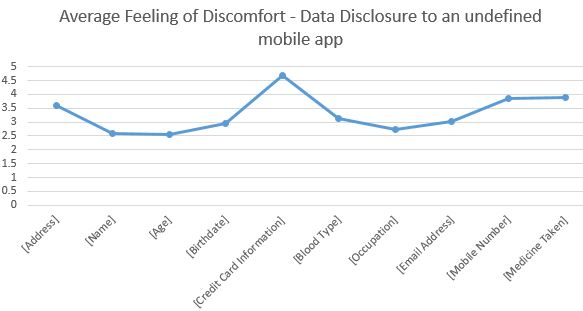
\includegraphics[width=0.5\textwidth]{Average_Generic}
\caption{Feeling of Discomfort in Disclosure - Undefined application}
\end{center}
\end{figure}

\begin{figure}[h]
\begin{center}
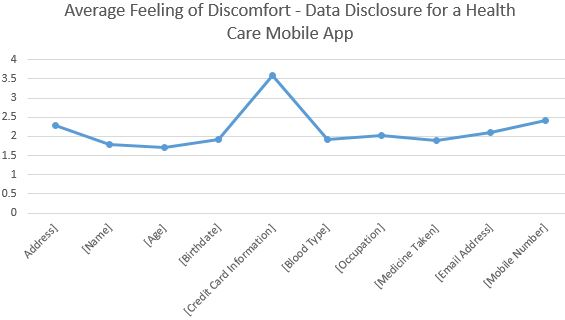
\includegraphics[width=0.5\textwidth]{Average_Health}
\caption{Feeling of Discomfort in Disclosure - Health  application}
\end{center}
\end{figure}

\begin{figure}[h]
\begin{center}
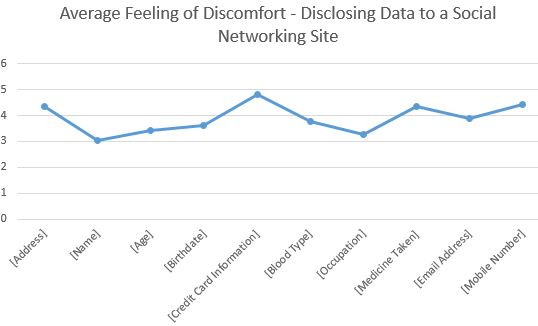
\includegraphics[width=0.5\textwidth]{Average_SocialNetworking}
\caption{Feeling of Discomfort in Disclosure - Social Networking application}
\end{center}
\end{figure}

\begin{figure}[h]
\begin{center}
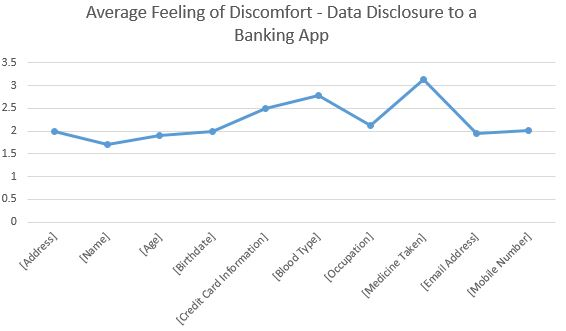
\includegraphics[width=0.5\textwidth]{Average_Banking}
\caption{Feeling of Discomfort in Disclosure - Banking application}
\end{center}
\end{figure}

It can be seen that irrespective of the context of disclosure, participants had a higher discomfort in disclosing their credit card number. This is because users consider their credit card number to be a highly sensitive data item.  Similarly we observed higher discomfort in disclosing medicine taken and blood type. However, the discomfort in disclosing the credit card number was very low for banking app because the credit card number is a data item that is relevant for the banking app. This suggests that users feel more comfortable sharing even sensitive data if the data item is relevant for the application. This observation is also observed with lowered discomfort in sharing medicine taken and blood type with a health care app.

Users demonstrated a relatively higher discomfort in sharing details with a social networking site. We defined the social networking site to have no control over data visibility once the data is disclosed. Therefore, we can assume that users have concern over data visibility when they disclose data into an application. 

In order to achieve the goals of the research, we calculate the effect of the variables we studies on the feeling of discomfort in disclosing data in the following subsections.

\subsection{Effect of data sensitivity to the feeling of disclosure -  $F_d,D_s$}

In order to calculate this we defined sensitive data from the 10 data items we provided the users following the definition for sensitive data in the data protection regulations [more details to be included]. We first calculated the feeling of disclosure of credit card\/name, blood type\/name and medicine taken\/name for all 151 participants and then averaged this across the 151 participants. Then we took the average of these three values as the average effect of sensitivity on data disclosure discomfort. The value we received was 1.790. 

We observed that the participants were most reluctant to disclose their credit card number which had an average effect of 2.33, followed by medicine taken with an average of 1.93. 

\subsection{Effect of data relatedness to the feeling of disclosure -  $F_d,D_r$}

In order to calculate the relatedness, we identified related data for the three application contexts we defined (disregarding the generic application context). We defined blood type to be related to the health care application, and medicine taken and blood type to be related to the health care app. We used the same data items in the social networking app as instances of disclosing unrelated data. The average effect of relatedness on data disclosure discomfort we received was 0.532, which suggests that users feel comfortable sharing data when the data item is related to the application. 

\subsection{Effect of data visibility to the feeling of disclosure -  $F_d,D_v$}
For this, we told the participants that the data visibility in the social networking app is not controllable for the user. That is they did not have control over who could see the data in the application. We also told them that the generic app had control for visibility. Then we compared the discomfort of sharing their age, address, email address and mobile number. We obtained the average effect of visibility on data disclosure discomfort as 2.66. This shows that users were more uncomfortable sharing their data in the event they had no control over the visibility over data. Compared to the other two factors (relatedness and sensitivity) users were most concerned about the visibility.


\subsection {Relationship among sensitivity, visibility and relatedness}

We observed that participants were most concerned about the visibility their data get in an application when they disclose data. $F_d,D_v(av)$ had a value of 2.66, where as $F_d,D_s(av)$ had a value of 1.790. Both sensitivity and visibility of data were directly proportional to the discomfort of data disclosure (effect $>$ 1). 

We calculated the relationship between sensitivity and visibility to be 1.48. That is users felt 1.5 times more uncomfortable sharing their data considering the visibility of the data item compared to the sensitivity of the data item. 

As expected, the relatedness of a data item to the application context was observed to be inversely proportional to the discomfort in sharing data items. The average effect of relatedness on discomfort of disclosing data had a value of 0.531 (effect $<$ 1).

Therefore, we define the relationship of data sensitivity, visibility and relatedness to the privacy risk associated with the data item for a given software system context as below,

\[ \text{Privacy Risk}  =
\frac{
      \text{Sensitivity} \times 1.5 \times \text{Visibility} }
 {
       \text{Relatedness }}
\]



\section{Discussion}

[to be decided]

\section {Limitations}

The study had several limitations. Firstly this was a remote survey. While remote surveys are beneficial in getting a large sample of participants in a relatively small period of time, direct engagement with users would disclose more in depth information when it comes to qualitative analysis. However, the main contribution of the paper was the derivation of the privacy measurement formula. Furthermore, for the qualitative component of data analysis we reached data saturation with the codes with 17 participants. The survey had 133 respondents which makes the results valid. Contextual studies involving real time applications that directly engage users in a natural setting could be used to observe how our findings stand in such setups.



\section{Conclusion and Future Work}



% Fonts specification --- not shown as it doesn't exist in the Word document either. 

%\section{Fonts}

%A summary of fonts is provided in Table \ref{tab: fonts}. 

%\begin{table}[thb]
%\centering
%\caption{\label{font-table} Font guide. \vskip 3pt }
%\label{tab: fonts}
%\begin{tabular}{l|rl}
%\hline \bf Type of Text & \bf Font Size & \bf Style \\ \hline
%paper title & 14 pt &  \bf bold \\
%authors & 10 pt &  \underline{email} underlined \\
%abstract title & 12 pt &  \bf bold\\
%abstract text & 10 pt &  \it italic\\
%section titles & 12 pt & \bf bold \\
%subsection titles & 11 pt & \bf bold \\
%document text & 10 pt  & \\
%captions & 9 pt & \sansserifformat{\captionsize sans-serif, \bf bold} \\
%bibliography & 9 pt & \\
%footnotes & 8 pt & \\
%\hline
%\end{tabular}
%\end{table}


\section{References} 

List and number all bibliographical references in 9-point Times, single-spaced, at the end of your paper. When referenced in the text, enclose the citation number in square brackets, for example \cite{Jones2015,Smith2015} and \cite{Smith2015}. Where appropriate, include the name(s) of editors of referenced books.

% if added before the last page, this command can help balancing columns
%\addtolength{\textheight}{-.2cm} 

%Bibliography 
\bibliographystyle{ieeetr}
\bibliography{sample}


\end{document}
